\documentclass{report}

\usepackage{textcomp}
\usepackage{graphicx}
\usepackage{fancyhdr}
\usepackage{subcaption}
\usepackage{multicol}
\usepackage{outlines}
%===================================
\newcommand{\classinfo}{{\bf Configuring VLANS \\ And Trunks}\\{\it CIT 167}\\{Chaz Davis}}
\newcommand{\semester}{BCTC \\ Spring 2020}
%===================================
\newcommand{\mysection}[1]{\section*{#1}}
\newcommand{\mysubsection}[2]{\textbf{\romannumeral #1) #2}}
%===================================
\setlength{\headheight}{15.2pt}
\pagestyle{fancy}
\fancyhf{}
\lhead{ \fancyplain{}{Chaz Davis} }
\rhead{ \fancyplain{}{\today} }
\cfoot{ \fancyplain{}{\thepage} }
\renewcommand{\headrulewidth}{0.5pt}
\renewcommand{\footrulewidth}{0pt}

%===================================
\title{\classinfo}
\author{\semester}
\date{\today}

%===================================

\begin{document}

\maketitle

%===================================
\mysection{\textbf{Part 1: Configuration}}

I set up the configurations for each pc on the network. I then copied and
pasted the commands from the handout for each of the switches.
The network is all up and running.

\begin{figure}[!h]
  \centering
  {\label{run13}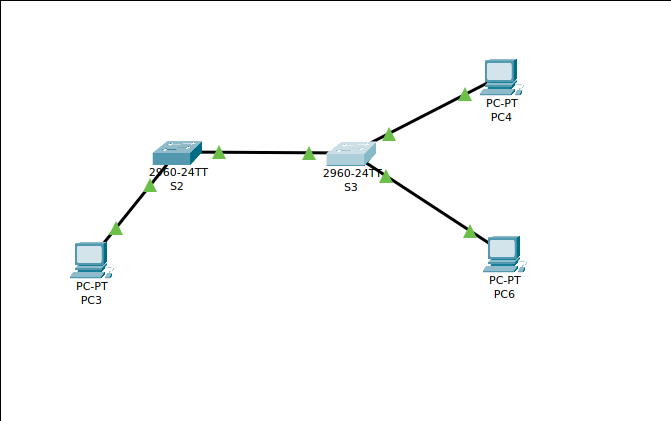
\includegraphics[width=.45\linewidth]{Figures/2020-03-08-183211_671x421_scrot.png}}
  \caption{The Network Up and Running}
\end{figure}


%===================================

\end{document}
